\section{Logical Modelling}\label{sec:lm}
The logical data model (LDM) is the conceptual data model's enlarged format. It describes how to set up a system that is not particular to any database. It primarily establishes the data elements and the relationships between them. A logical data model is the foundation of the physical data model (FDM). Attributes, primary keys, foreign keys, relationship cardinality, and descriptive entities and classes are all described in an LDM. This data model clearly defines all of the relationships between the entities. As a result, anyone may convert an LDM to an FDM in any database management system. This data model is often created by data architects and business analysts.\\

\begin{figure}[H]
	\captionsetup[subfigure]{labelformat=empty}
	\hfill
		\subfloat{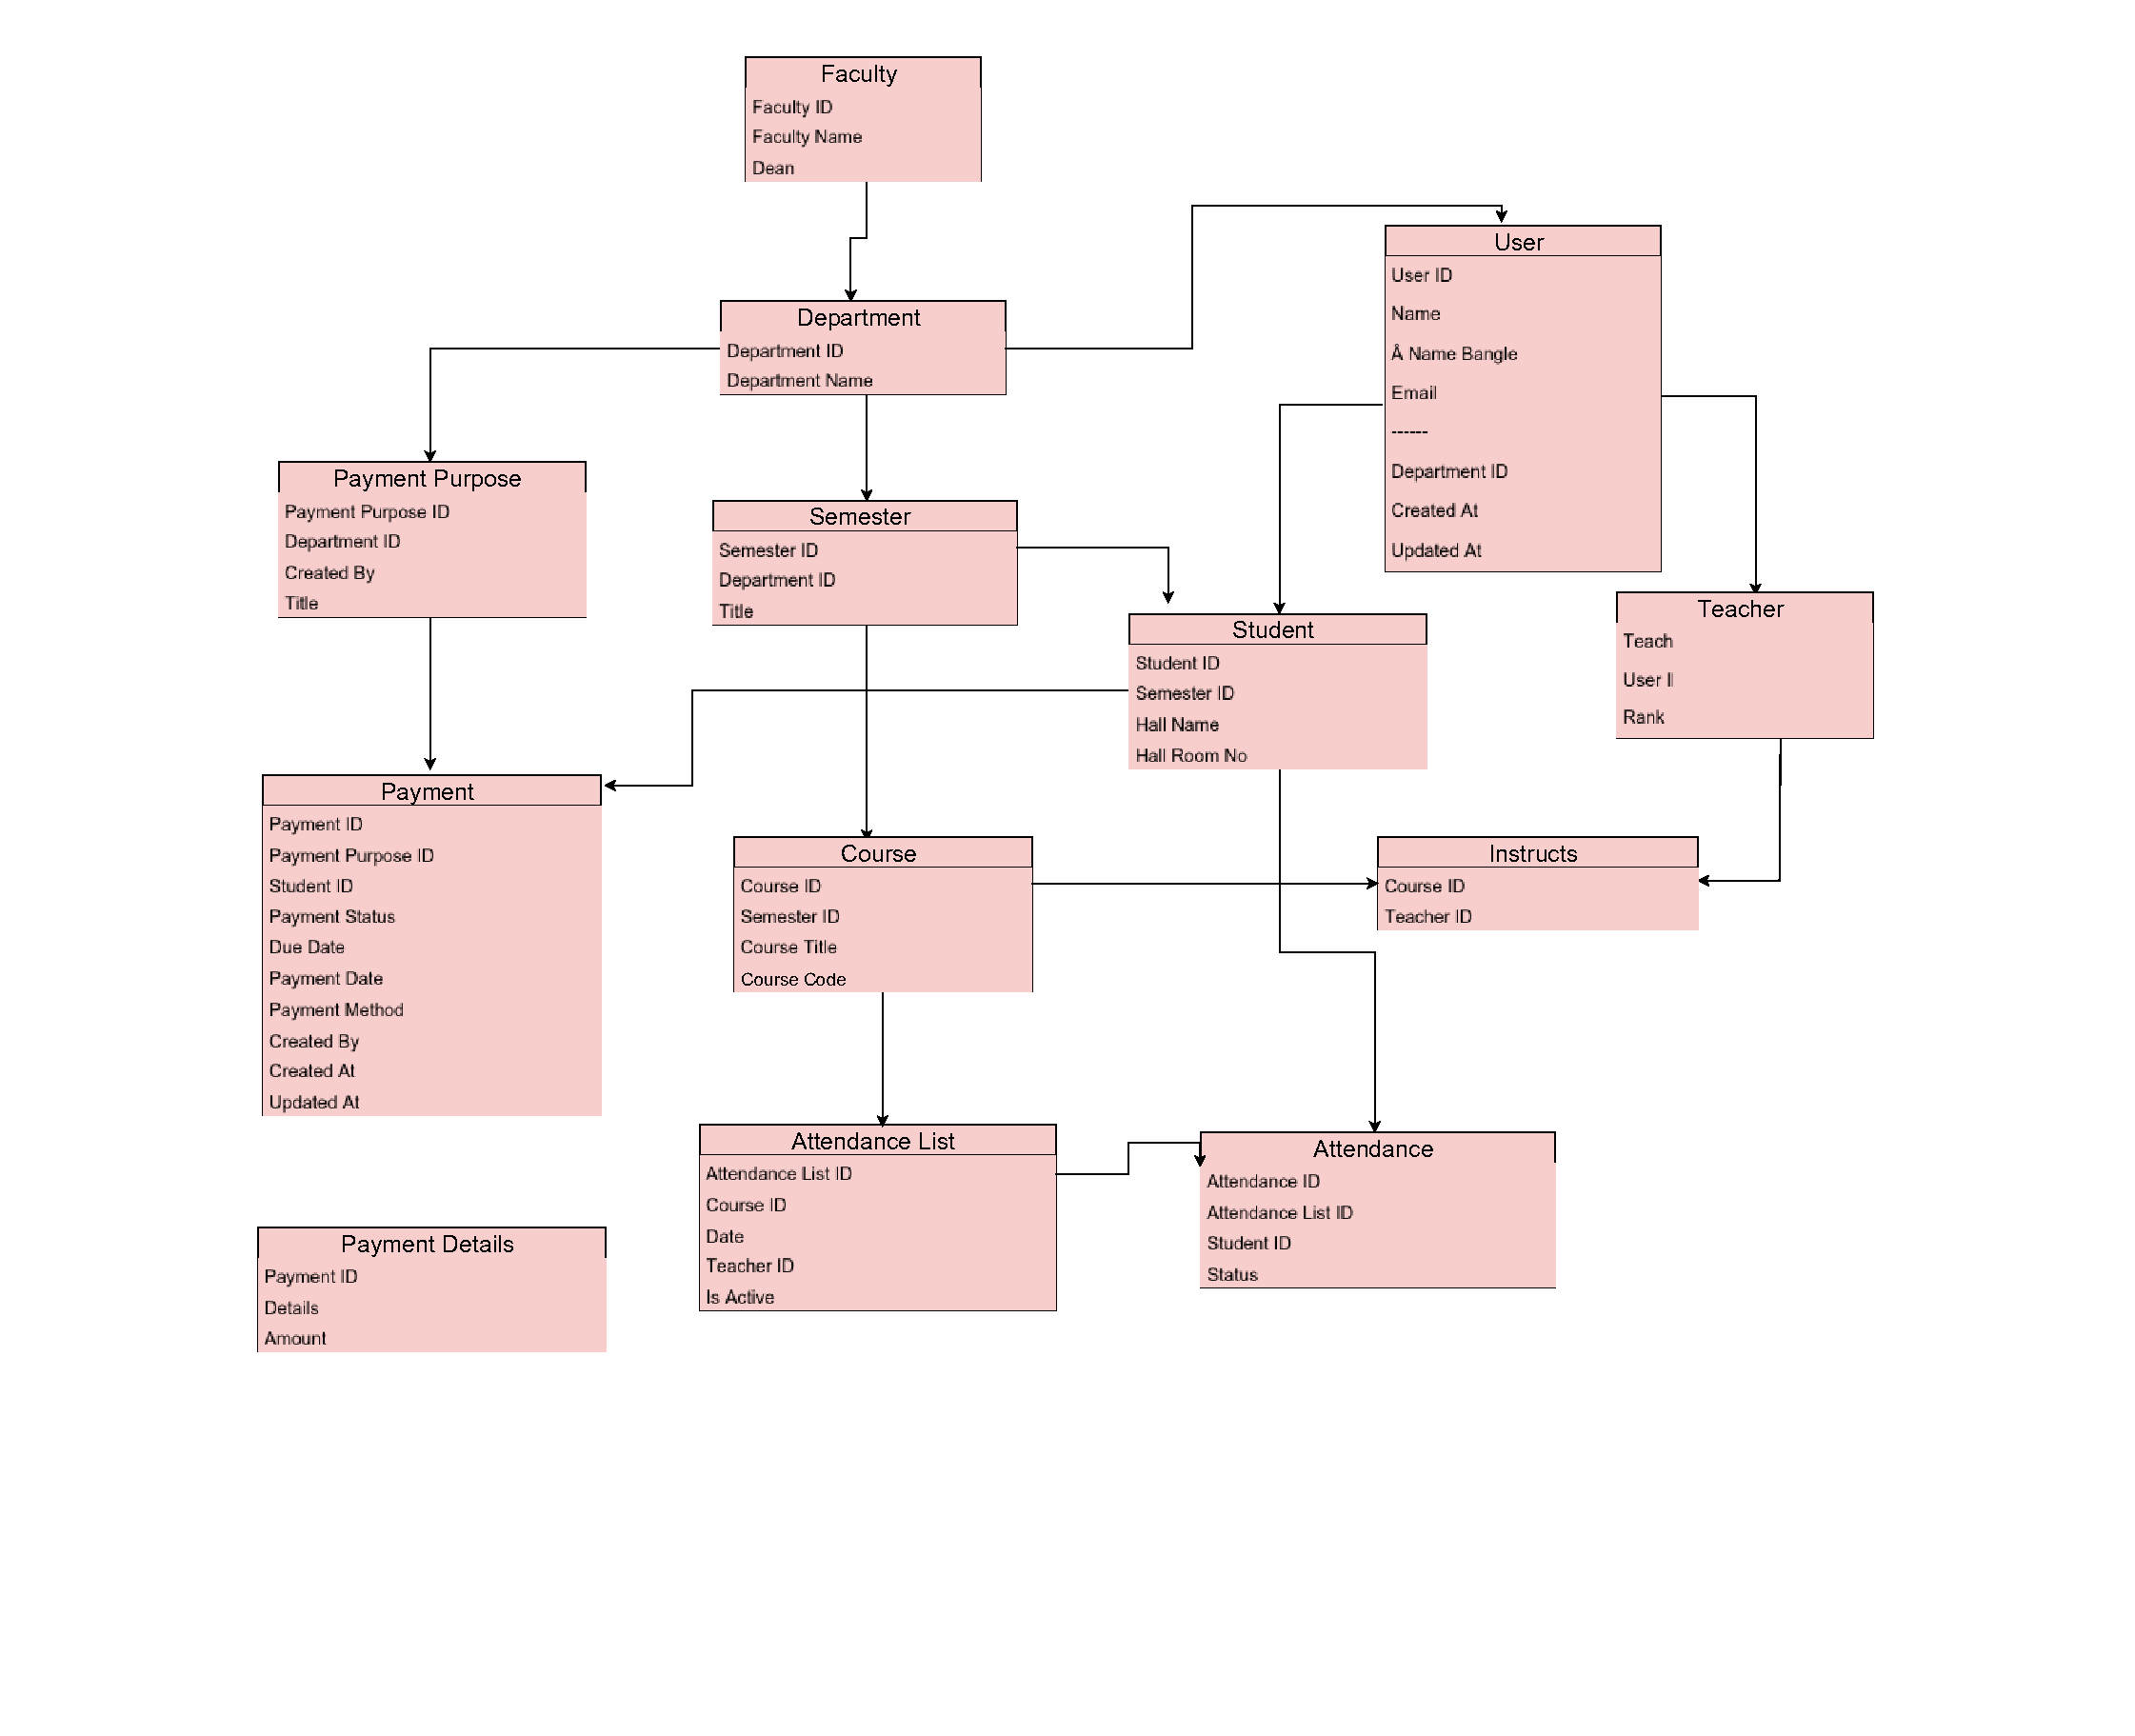
\includegraphics[width=0.7\textwidth]{images/logical}}
	\hfill
		\subfloat{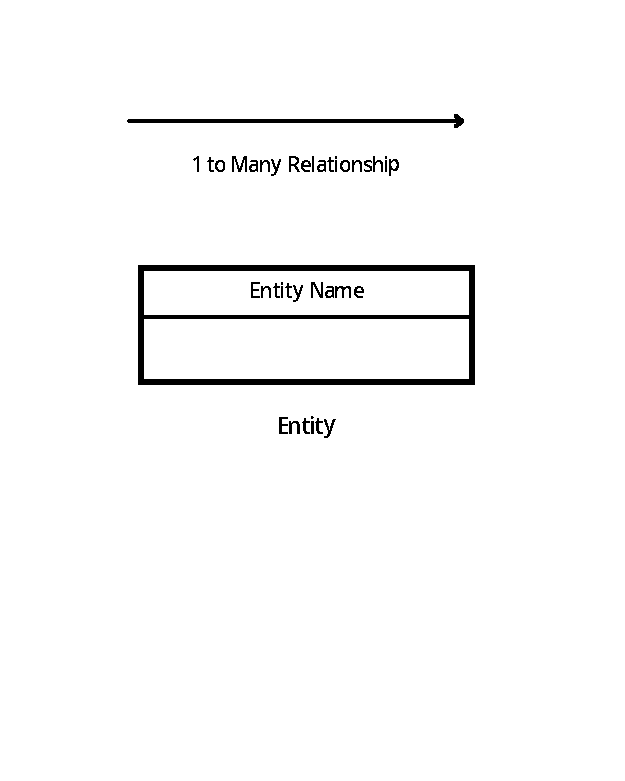
\includegraphics[width=0.3\textwidth]{images/legend}}
	\hfill
	\caption{Logical Data Model of CU-OPAS}
\end{figure}
Write a short description of Relation model. 
Write a how you convert your E-R model in Relational model
\clearpage